\section{Using Instance Pointcuts with Design Patterns}

Instance pointcuts offer a new way of modularizing objects; this new modularization method can be used in conjuction with design patterns for a well-localized implementation and fine-grained assignment of object roles. 
In this section we will discuss how instance pointcuts improve the implementation of design patterns.
We will go over three scenarios which use factory, adapter and observer patterns respectively.

Let us first introduce the example setting for the different scenarios.
We have a simple drawing application which can be used to draw basic shapes. 
The user selects a certain shape, which appears in the middle of the screen. 
Then the user can scale, move and color the shape as she pleases.
The shape objects adhere to the hierarchy shown in figure~\ref{fig:shapeshier}.


\begin{figure}
\centering
 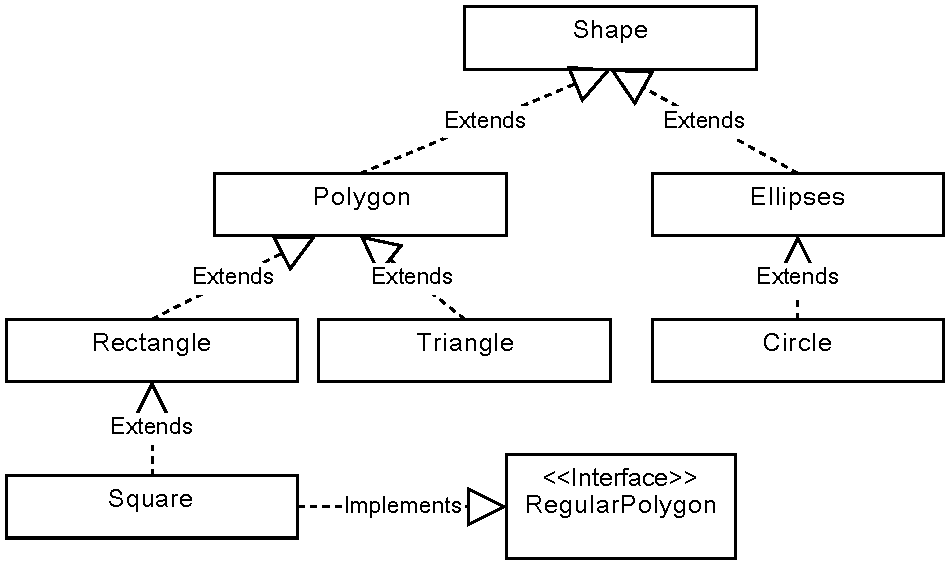
\includegraphics[width=0.7\textwidth]{images/shapes.pdf}
 \caption{The shapes hierarchy}
 \label{fig:shapeshier}
\end{figure}

The \lstinln{Shape} class is an abstract class, and root of the shapes hierarchy. 
The hierarchy contains two types of shapes, \lstinln{Circle} and \lstinln{Polygon}.
The \lstinln{Polygon} class have common shapes as concrete subclasses, \lstinln{Triangle} and \lstinln{Rectangle}, the latter has a subclass called \lstinln{Square} which implements the \lstinln{RegularPolygon} interface.
Each concrete shape object is created by a factory class that implements the abstract factory \lstinln{ShapeFactory}. 
The \lstinln{ShapeFactory} interface contains a single method called \lstinln{createShape} which returns a \lstinln{Shape} object.
According to the selection made in the application GUI, the corresponding shape factory's \lstinln{createShape} method is invoked.
For example if the user selects the shape circle, then the \lstinln{CircleFactory}'s creation method is called and the returned object is drawn on the screen. 

\subsection{Scenario 1 -- Factory Pattern}
In this scenario we would like to extend our application with the following feature; when the user selects a certain type shape and presses the button ``count'', the application will display how many shapes of that type is currently in the canvas. 

With the current implementation, each shape that is drawn is kept in a list called \lstinln{shapes<Shape>}.
In order to count, for example, \lstinln{Circle} objects, we need to add the code shown in listing~\ref{lst:countcircles}.
This code counts the \lstinln{Circle} objects in the list \lstinln{shapes}, every time the a circle is selected and the count button is pressed.
In order to count for different shapes, we need to add additional if statement to identify the type of the selected shape. 

\begin{lstlisting}[float, label={lst:countcircles}, caption={A code snippet for counting \lstinln{Circle} objects}]
int count = 0;
if(selected.isCircle())
  for(Shape s: shapes)
    if(s instanceof Circle) ~\label{lst:cc:io}~
      count++
\end{lstlisting}

Rather than counting everytime the count button is pressed, we can also keep track of the number of the objects in designated variables. 
For example, we can have an static integer field called \lstinln{circleCount}.
Whenever the \lstinln{CircleFactory} creates a new \lstinln{Circle} it can increment this value with the following statement \lstinln{Canvas.circleCount++}.
In the event of deleting a \lstinln{Circle} object, the method \lstinln{delete()} is called on the object. 
So inside the delete method of the \lstinln{Circle} class we must call \lstinline~Canvas.circleCount--~.
This is obviously a scattered implementation of the counting feature. 

With instance pointcuts we can localize the counting operation by creating an instance pointcut for each shape. 
An example is shown in listing~\ref{lst:counrcirclesipc}. 
The instance pointcut \lstinln{circles} is responsible for keeping a set of \lstinln{Circle} objects, while the life-cycle phase for each object is marked by its creation (line~\ref{lst:ccipc:creation}) to its deletion (line~\ref{lst:ccipc:deletion}).
Using this instance pointcut, the number of \lstinln{Circle} objects can be obtained by \lstinln{[Aspect].circles().size()}.

\begin{lstlisting}[float, label={lst:countcirclesipc}, caption={An instance pointcut that keeps track of \lstinln{Circle} objects}]
static instance pointcut circles<Circle>: 
  after(* CircleFactory.createShape(..) && returning(instance)) ~\label{lst:ccipc:creation}~
  UNTIL
  after(* Circle.delete() && target(instance)); ~\label{lst:ccipc:deletion}~
\end{lstlisting}

Modularizing the shape groups concern in instance pointcuts is also beneficial for possible future extensions.
For example we want to extend our application with a selection feature as follows; when the user selects a single shape object and double clicks on it, then the other objects which are of the same type must be selected. 
If the user performs this operation on a circle shape, we can retrieve the set of objects maintained by \lstinln{circles} instance pointcut and iterate over it to set the field \lstinln{selected} to \lstinln{true}.

Another case when the information about the origin of the object creation bears a significance is when there are multiple ways of creating an object; for example when there are multiple factory classes or methods which create a differently configured version of objects of same type.  


\begin{lstlisting}[float, label={lst:countcircles}, caption={Extended code snippet for counting textured or colored \lstinln{Circle} objects}]
int count = 0;
if(selected.isCircle())
  for(Shape s: shapes)
    if(s instanceof Circle) ~\label{lst:cc:io}~
      {
	 if(s.getFilling() instanceof Texture) ~\label{lst:cc:iot}~
	  count++
      }
\end{lstlisting}

For example, assume we have replaced the \lstinln{CircleFactory} class with two new factory classes called \lstinln{TexturedCircleFactory} and \lstinln{ColoredCircleFactory}, which create \lstinln{Circle} objects with different values for the \lstinln{filling} field.
Going back to the shape counting example discussed above, let us consider once again listing~\ref{lst:countcircles}. 
Here the \lstinln{instanceof} check on line~\ref{lst:cc:io} cannot distinguish between a \lstinln{Circle} object that is textured or colored.
So if we would like to count textured circles, we need to extend this code as shown in listing~\ref{lst:countcircles:ext}.
On line~\ref{lst:cc:iot} we perform an additional check to see if the \lstinln{filling} of the \lstinln{Circle} object is an instance of the type \lstinln{Texture}.
An instance pointcuts solution would be a slight modification of the instance pointcut shown in listing~\ref{lst:countcirclesipc}; instead of selecting the join-points at \lstinln{CircleFactory.createShape}, we select \lstinln{TexturedCircleFactory.createShape}. 

In this scenario we have shown that instance pointcuts can be used in conjunction with the factory pattern to capture the information ``by which factory an object was created''.
We have discussed two benefits; the localization of concerns by using the modularization offered by instance pointcuts and capturing information about the configuration of the object by looking at its origin of creation.


\subsection{Scenario 2 -- Adapter Pattern}

In this scenario, we want to add the export feature to out drawing application to a different file format.
The new file format can only support non-textured shapes with four edges or more, so even if we have drawn circles in a drawing, we cannot save them as circles.
It is also not possible to save the triangles, because of the four edges limitation. 
If the user chooses to do so, she can save them as squares which have the same edge size as the diameter of the circle.


In order to implement this feature we need to single out non-textured rectangles (including squares) and we need to adapt the non-textured \lstinln{Circle} objects to \lstinln{Square} objects, to save them.
Listing~\ref{lst:circle2square} shows a simple \lstinln{Circle} to \lstinln{Square} object adapter.

\begin{lstlisting}[float, label={lst:circle2square}, caption={An adapter for creating a \lstinln{Square} object by wrapping a \lstinln{Cicle} object}]
public class Circle2SquareAdapter extends Square
{
  Circle adaptee;
  public Circle2SquareAdapter(Circle adaptee)
  {
    this.adaptee = adaptee;
  }
  @Override
  public double getEdgeLength()
  {
    return adaptee.getDiameter()
  }
}
\end{lstlisting}


Since we can only save a specific set of objects, i.e non-textured polygons which have more than four edges, we need to filter these object from the canvas that is being exported.
The first instance pointcut shown in listing~\ref{lst:nts} keeps a set of non-textured objects.
The following two instance pointucts refines this set according to type; \lstinln{nonTexturedCircles} selects non-textured \lstinln{Circle} objects and \lstinln{nonTexturedRect} keeps non-textured \lstinln{Rectangle} objects.


\begin{lstlisting}[float, label={lst:nts}, caption={Instance pointcuts that select non-textured shapes in the canvas}]
static instance pointcut nontexturedshapes<Shape>: 
  after(* Shape.new(..) && returning(instance) && !within(* Textured*Factory)) 
  UNTIL
  after(* Shape.delete() && target(instance));
static instance pointcut nonTexturedCircles<Circle> : nontexturedshapes<Circle>;
static instance pointcut nonTexturedRect<Rectangle> : nontexturedshapes<Rectangle>;
\end{lstlisting}





\begin{lstlisting}[float,  caption={Adapting non-textured \lstinln{Circle} objects to \lstinln{Square} objects}, label={lst:adapt:c2s}]
static Map<Circle, Square> c2sMap = new HashMap<CircleSquare>();~\label{lst:adapt:map}~

after(Circle c): nonTexturedCircles_instanceAdded(c); ~\label{lst:added:b}~
{
  c2sMap.put(c, ((Square)new Circle2SquareAdapter(c)));
}~\label{lst:added:e}~
after(Circle c): nonTexturedCircles_instanceRemoved(c)~\label{lst:rem:b}~
{
  c2sMap.remove(c);
}~\label{lst:rem:e}~
public static Collection<Square> getAdaptedCircles()
{
  return c2sMap.values();
}
\end{lstlisting}

Note that the non-textured \lstinln{Circle} objects should be adapted before the export operation.
By using the monitoring features of instance pointcuts, we can create the adapted values inside the same aspect that contains the instance pointcuts mentioned above.
In listing~\ref{lst:adapt:c2s} an implementation that uses \lstinln{Circle2SquareAdapter} is shown. 
In this implementation we create a \lstinln{Map} called \lstinln{c2sMap} (line~\ref{lst:adapt:map}) that will hold the \lstinln{Circle} objects on the canvas and their corresponding \lstinln{Square} represenation using the \lstinln{Circle2SquareAdapter}.
In order to populate this map we use the \lstinln{nonTexturedCircles_instanceAdded} pointcut, which is readily available with the definition of \lstinln{nonTexturedCircles}.
In the after advice that uses this pointcut (lines~\ref{lst:added:b}--~\ref{lst:added:e}) performs the following operation; when a new \lstinln{Circle} object is added to the canvas, a new \lstinln{Square} object is created by adapting this \lstinln{Circle} object.
Then these objects are added to the map, \lstinln{Circle} object as the key and \lstinln{Square} object as the value.
The \lstinln{nonTexturedCircles_instanceRemoved} pointcut is used to remove the mappings from \lstinln{c2sMap} (lines~\ref{lst:rem:b}--~\ref{lst:rem:e}). 
Finally we create the static method \lstinln{getAdaptedCircles} to return the adapted values currently contained in the map \lstinln{c2sMap}.
Using these instance pointcuts and the extra code shown in listing~\ref{lst:adapt:c2s}, we can implement the export function as shown in listing~\ref{lst:export}.

\begin{lstlisting}[float,  caption={The export function}, label={lst:export}]
public void export()
{
  List<Rectangle> 2bExported = new ArrayList<Rectangle>();
  2bExported.addAll([Aspect].nonTexturedRect());
  2bExported.addAll([Aspect].getAdaptedCircles());
  Exporter.export(2bExported);
}
\end{lstlisting}

In this scenario we have selected a specific set of objects and adapted them with a given object adapter.
Instance pointcuts provided us with the expressive power over selecting specific objects as adaptees.
Also we localized the adaptation concern to the aspect, which prevented a possible tangling in the export function.


\subsection{Scenario 3 -- Observer Pattern}
Our final scenario shows how instance pointcuts can help localize the assignment of the role of \emph{being observed} to an object.
In this scenario we want to observe the color change events of \lstinln{Triangle} objects.
Using instance pointcuts we can select the set of colored \lstinln{Triangle} objects as shown in listing~\ref{lst:tricolor} (lines~\ref{tricolor:ip:b}--~\ref{tricolor:ip:e}).
We monitor the addition of colored triangles to the canvas with the \lstinln{triColor_instanceAdded} pointcut (line~\ref{tricolor:after}). 
To each colored triangle, we add the \lstinln{ColorChangeObserver} after it is added to the canvas (line~\ref{tricolor:addobs}).


\begin{lstlisting}[float, label={lst:tricolor}, caption={An instance pointcut that keeps track of colored \lstinln{Triangle} objects}]
static instance pointcut triColor<Triangle>: ~\label{tricolor:ip:b}~
  after(* ColoredTriangleFactory.createShape(..) && returning(instance))
  UNTIL
  after(* Triangle.delete() && target(instance));  ~\label{tricolor:ip:e}~
  
after(Triangle t): triColor_instanceAdded(t) ~\label{tricolor:after}~
{
  t.addObserver(new ColorChangeObserver()); ~\label{tricolor:addobs}~
}
\end{lstlisting}

Once again instance pointcuts provide expressive power over the choice of objects that is observed.
Also it localizes the code for adding an observer to the observer list of an object, in an aspect. 
The advantage is a fine-grained management of objects in the application and the prevention of implementation related issues that comes with using the observer design pattern.











